%------------------------------------------------------------
%
\documentclass{llncs}%
\usepackage{quotes}
\usepackage{epstopdf}
\usepackage{bsymb}
\usepackage{alltt}
\usepackage{amsmath}%
\usepackage{graphicx}
\usepackage{hyperref}
\usepackage{enumitem}
\usepackage{amssymb,amsfonts,textcomp}
\usepackage{color}
%-------------------------------------------
\begin{document}
%
\title{Using Templates for Configuration\\ in Event-B Code Generation}

\author{A. Edmunds}

\institute{University of Southampton, UK}

% Templates
% Interface
\maketitle
%
\begin{abstract}
The Event-B method, and  its tools, provide a way to formally model systems; Tasking Event-B is an extension facilitating code generation.  We have recently begun to explore how we can configure the code generator, for deployment with different targets. In this paper, we describe how templates can be used, to avoid hard-coding `boilerplate' code, which is not directly associated with the formal model, but is target specific. We have developed a lightweight approach, where tags (i.e. tagged mark-up) can be inserted in the source templates. Template processing involves copying code, verbatim, from the source to the target unless a tag is encountered. Tags can be used to inject source code, or produce meta-data output, using custom code generators. This is an extensible approach, which makes use of the Eclipse extension-point mechanism. The template-processors can be used with any text input file; and was used in a C code generator, which we use as a running example in the paper. 
 \end{abstract}
%
%
\section{Introduction}
%
Rodin is a  tool platform~\cite{abrial10rodin} for the rigorous specification of critical systems, using the Event-B approach~\cite{ABR10}. The tool was developed in the RODIN project~\cite{RodinTool}, and experience with industry was gained in the DEPLOY project~\cite{DEPLOY}. Tasking Event-B~\cite{Edmunds2009,Edmunds2008,ae2011a,ae2012b} is an extension to Event-B that facilitates generation of source code; code generators are currently available for Java~\cite{JavaSpec}, Ada~\cite{ada2005}, C for OpenMP~\cite{openmp}, and C for the Functional Mock-up Interface~\cite{FMISTD} standard. 

The work reported in this paper has been undertaken during the ADVANCE project~\cite{advance}; a continuation of the Event-B research effort, this time focussing on co-simulation of Cyber-Physical Systems. However, the initial discussion and some of the ideas arose from an industrial collaboration with Thales Transportation Systems, Germany; during which time we undertook a case study, involving a top-to-bottom appraisal of the Event-B approach - from abstract specification to implementation. One of the main issues of concern was that of generation-time configuration for particular deployments.  This paper introduces an approach that allows configuration, before code-generation, for particular target environments. It is envisaged that this is just one part of a methodology, that would be necessary for such configuration, in an industrial strength tool.   

Often, when a software system is being implemented, there is a large amount of code that is common to the particular target implementation. Examples of this might be code for system life-cycle management, system health monitoring, or task scheduling. But, this code is independent of the actual state and behaviour of the part of the system being formally modelled. To achieve this we have provided a simple Eclipse extension, to allow the use of templates with tagged mark-up. The templates can contain the boilerplate code, and insertion points for model-specific, generated code. The use of templates should facilitate re-use of existing code, and importantly, avoid having to hard-code such details. It can also provide a focal point for applying configuration criteria; something that can be explored in future work. It is envisaged that the template writer will be working on models nearing the end of the development process, close to the implementation-level. So they will, at least, require knowledge of the link between model and code. The template writer will need to apply annotations to the boiler-plate code by adding annotations in the form of tags. The tags can define locations where other templates should be expanded. They also define code insertion points, and meta-data generators, linked to pre-configured code fragment-generators. We discuss these features in Sect.~\ref{templates}. This template-based approach is suitable for use with any textual source and target file. We have recently undertaken work to provide a C code generator for use with the Functional Interface Standard (FMI)~\cite{bloch2012,bloch2011,FMISTD}. We made use of the template-based approach for this; but it was also our aim to make the template mark-up, and code fragment-generators, customizable, extensible and suitable for use with other text based input. We provide an overview of FMI is Sect.~\ref{FMI}, an overview of Event-B in Sect.~\ref{EB}, and code generation with Tasking Event-B in Sect.~\ref{TEB}. We introduce templates, and show an example of their use, in Sect.~\ref{templates}, and conclude in Sect.~\ref{conc}.
%
%
\section{An Overview of FMI}\label{FMI}
%
In order to provide a context for the use of templates, we base the discussion around the work undertaken on the Event-B-to-FMI translator. It is therefore necessary to provide some background on the Functional Mock-Up Interface (FMI) standard~\cite{bloch2012,bloch2011,FMISTD}; a tool-independent standard, developed to facilitate the exchange, and re-use, of modelling components in the automotive industry. It is a C-based standard, defining an interface for re-usable components, known as Functional Mock-up Units (FMUs). FMUs play the role of slave simulators in simulations that are coordinated by a simulation master. The master simulator is not defined in the FMI standard, but its job is to coordinate the simulation e.g. by stopping and starting slaves. It also manages the communication; where all the slaves' input and output values are communicated via the master, never directly between slaves. 

In the early stages of an Event-B development, co-simulation can be performed using discrete Event-B models, and continuous (FMU) models of the environment. At some point it may be desirable to replace the discrete Event-B models, with discrete (FMU) implementations. The implementations can then be used in the simulation as a more accurate representation of the deployed system, and they can be used to test the implementation with a continuous model of the environment. To target the FMI co-simulation framework, we generate code for an FMU from the Event-B model. An FMU is a compressed file, the contents of which is defined in the FMI standard. The FMU should contain an XML description of the model being simulated, and include the shared libraries required to run the simulation. The shared libraries are compiled from the C code that we generate from Event-B. To conform to the FMI standard, FMU implementers must implement API functions for simulation life-cycle management, such as instantiating a slave, initialising a slave's variables, and terminating the slave. Many of the functions defined in the API are not dependent on the particular model being simulated, the code is the same for all models. We wish to avoid hard-coding the translation where possible; so, the use of templates provides a good solution. Since, this code is common to a particular platform it provides the opportunity to apply configuration data, for that platform.   
%
\section{An Overview of Event-B}\label{EB}
%
The Event-B method~\cite{ABR10} was developed by J.R. Abrial, and uses set-theory, predicate logic and mathematical constructs to model discrete systems. Event-B \emph{machines} are used to describe dynamic properties of a system, and \emph{contexts} describe fixed properties. Properties (such as safety-properties) are described in a machine's \emph{invariants} and a context's \emph{axioms}. 

An example of an Event-B machine can be seen in Fig.~\ref{fig:controllerSpec2}, which shows an abstract model of the pump controller from our case study. We ultimately use this model to generate code for use in an FMU; but we present the details here, only to illustrate our explanation of Event-B. We will not require in-depth understanding of the model itself, but we will refer to entities such as machines, variables, and a common language model (CLM) that we will explain in due course.  But first we provide some details of the discrete \emph{pumpController} model, that we would like to use in a co-simulation. The model describes a system where the controller receives a value of the fluid level, and whether a user-request to turn the pump on has been detected. Based on the known conditions, a command to turn the pump on may be issued, or a warning is issued if a minimum level \emph{MIN} has been reached.    
%
%
\begin{figure}
\centering
\begin{minipage}{0.95\textwidth}
\textcolor{blue}{MACHINE} m1 \textcolor{blue}{REFINES} m0 \textcolor{blue}{SEES} ctx \\
\textcolor{blue}{VARIABLES} \text{m\_level, c\_level, e\_level, m\_pumpOnReq, c\_pumpOnReq, e\_pumpOnReq,} \hspace*{0.2cm} m\_pumpOnCmd, c\_pumpOnCmd, e\_pumpOnCmd, m\_warn, c\_warn, e\_warn,\\
\hspace*{0.2cm} c\_level\_internal, c\_pumpOnReq\_internal\\
\textcolor{blue}{INVARIANTS}\\
\hspace*{0.2cm}(c\_level\_internal $\leq$ MIN $\land$  c\_pumpOnReq\_internal = TRUE $\limp$  c\_warn = TRUE)\\
\hspace*{0.2cm} $\land$ (c\_level\_internal $>$  MIN $\land$  c\_pumpOnReq\_internal = TRUE\\
\hspace*{0.5cm} $\limp$  c\_pumpOnCmd = TRUE)\\
\hspace*{0.2cm} $\land$ (c\_level\_internal $\in  \intg$)\\
\hspace*{0.2cm} $\land$ (c\_pumpOnReq\_internal $\in$  BOOL) \ldots\\
\textcolor{blue}{EVENTS}\\
\textcolor{blue}{INITIALISATION} c\_level :=  100 $\pprod$ m\_level := 80 $\pprod$ c\_pumpOnReq :=  FALSE $\pprod$ \ldots\\
\textcolor{blue}{EVENT} fmiSetBoolean\_c \textcolor{blue}{REFINES} fmiSetBoolean\_c\\
\hspace*{0.2cm}\textcolor{blue}{ANY} p\\
\hspace*{0.2cm}\textcolor{blue}{WHERE} p = c\_pumpOnCmd $\land$ p $\in$ BOOL  \\
\hspace*{0.2cm}\textcolor{blue}{THEN} m\_pumpOnCmd :=  p\\
\hspace*{0.2cm}\textcolor{blue}{END}\\
\ldots
\end{minipage}
\caption{An Event-B  Pump Controller Model}
\label{fig:controllerSpec2}
\end{figure}
%
%

 In Fig.~\ref{fig:controllerSpec2}, we see that the machine \emph{refines} another machine, we will return to this aspect later in the section. Next we look at the \emph{sees} clause, it has a context (potentially it can have more than one). The context may contain sets, constants, axioms and theorems. In the case study we have a constant integer \emph{MIN}, defined in an axiom $MIN \in \intg$. Machines describe the dynamic aspects of a system, using state variables and guarded atomic \emph{events}. Events may have parameters, which model local variables, or incoming/outgoing parameter values. Variables are introduced in the \emph{variables} clause, and typed in the \emph{invariant} clause. The invariant also describes a required safety property, that if the level is at or below \emph{MIN}, and a user's pump-on request is detected, then a warning will be issued. The state \emph{pumpOnCmd = TRUE} is set, if the level is OK, and a pump-on request has been received.

In the next section we look at the \emph{Events} clause. Events describe state transitions, using action expressions; and the conditions under which they may occur, using guard predicates. An \emph{initialisation} event is a special unguarded event, that takes place before all other events. It describes the initial state of the machine, and occurs before all other events. After initialisation, any event with all its guards evaluating \emph{true} may occur. Actions (in the \emph{then} clause) contain assignment expressions. They can be deterministic or non-deterministic, $\bcmeq$ or $\bcmin$ resp. or the clause may even be empty, and do nothing (\emph{skip}). In the example, the \emph{fmiGetBoolean\_c} event refines the abstract \emph{fmiGetBoolean\_c} event. It declares a parameter \emph{p}, which is typed in the guard (\emph{where} clause). The other guard relates a parameter to a state variable $p = c\_pumpOnCmd$, which we use to model information passing between components in the system. Here the master receives the controller’s command to turn the pump on. In the example, variables prefixed \emph{m\_} identifies those of the master, \emph{c\_} the controller's, and \emph{\_e} the environment. Together, the guard and action refine \emph{m\_pumpOnCmd = c\_pumpOnCmd}. In a later step we will decompose \emph{m\_pumpOnCmd} and \emph{c\_pumpOnCmd} into separate machines. In the next subsections we briefly introduce refinement and decomposition.

\subsection{Refinement}
Refinement is the process of adding detail to a development, as we move towards implementation. A refinement machine can introduce new variables, invariants, and events. New, and existing events, can modify new variables; but, there are restrictions on how existing variables are modified. Consistency in the relationship between an abstract machine and its refinements is maintained by discharging the automatically generated proof obligations. Proof obligations represent the conditions that should be satisfied to demonstrate that the model is consistent with the specified properties. Discharging proof obligations demonstrates that the related properties hold. In many cases proof obligations are discharged by Rodin's automatic proof tools, but it is often necessary to perform interactive proof within Rodin. Interactive proof is undertaken by suggesting strategies, and sub-goals in the form of hypotheses. 

\begin{figure}
\centering
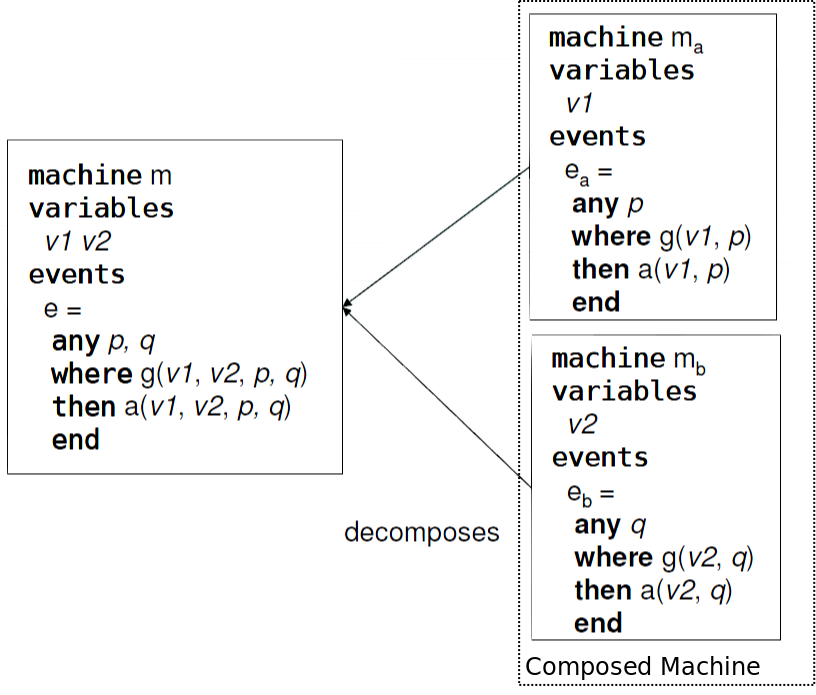
\includegraphics[width=0.6\textwidth]{Decomp2.png}
\caption{Shared Event Decomposition}
\label{fig:Decomp2}
\end{figure}

\subsection{Decomposition}\label{decomp}
Shared Event-B decomposition~\cite{Butler09a,decomp2010b} is a technique that we use to handle complexity; we are able to split a single machine specification into several. We begin with partitioning variables into machines. After decomposition the events that refer to them are shared between machines. A record of the composition is stored in the \emph{Composed machine} Event-B component~\cite{decomp2010c} as indicated in Fig.~\ref{fig:Decomp2}.  The shared events are said to synchronize: i.e. they are only enabled when the guards of each of the composed events are true.  The diagram shows an event $e$, which is decomposed, into $e_a$ and $e_b$.
%
%
%
In~\cite{ae2011a} we describe the synchronization of two events as being equivalent to a single, merged, atomic event, and then translated to a subroutine call, and subroutine definition. Event Synchronization may use shared parameters to facilitate communication between machines.   As we move towards towards implementation, the decomposed artefacts reflect entities in the implementation; which assists with code generation.

\section{Tasking Event-B}\label{TEB}
Tasking Event-B~\cite{ae2011a} is an extension to the Event-B language; an implementation-level, specification language. When annotations are added to a machine, it provides additional information which is used to assist in code generation. When translating to code, it is usually necessary to work with a subset of implementable Event-B constructs. We consider \emph{implementable constructs} to be those that are available in (or map well to) a programming language. We would therefore usually not consider non-deterministic assignment to be implementable, for instance, and add a restriction; that these are `refined out' of the implementation-level model. Annotations are added to both machines and contexts. The annotations are also used to generate an Event-B model of the implementation. 

Machines can be implemented as task/thread-like constructs; shared, monitor-like constructs; or provide simulations of the environment.  The machine \emph{Type} annotations are \emph{Autotask}, \emph{Shared} and \emph{Environ} respectively.  In embedded systems, \emph{autotask} Machines typically model \emph{controller} tasks (of the implementation). We impose restrictions on the communication between these machines. The aim is to simplify the mapping to implementations that prevent interference in multi-threaded deployments. We stipulate that \emph{autotask} machines cannot have synchronizing events, such as those arising from decomposition as described in Subsect.~\ref{decomp}. If communication is required between tasks in an implementation then a shared machine must be used, to model a protected object. This approach was influenced by the Ravenscar profile~\cite{Burns1999} for safe multi-tasking. Now, when it comes to generating code for an FMU, we do not have the same restriction, since the FMI master coordinates the interactions in such a way that interference is not possible. So in this case, events of \emph{autotask}'s may synchronize.

We now describe some of the Tasking Event-B constructs. The main behaviour of a system's  long-running task-like (or thread-like) processes are modelled by \emph{autotasks}. An annotation is applied using the usual user interface, to a standard Event-B machine, to indicate that it models an \emph{autotask}. An \emph{autotask} machine has a task body which contains flow control (algorithmic) constructs; \emph{Sequence}, \emph{Branch}, \emph{Loop}, \emph{Event}, \emph{EventSynch}, \emph{Event}. The syntax of the \emph{Task body} follows,
%
%
\begin{center}
\begin{minipage}{0.7\textwidth}
Task Body ::= TaskBody~ \textbf{;}~ TaskBody\\
\hspace*{1cm}$\pprod$ \textbf{IF}~ Event~ [\textbf{ELSEIF}~ Event~]$^*$~ \textbf{ELSE}~ Event~\textbf{END} \\
\hspace*{1cm}$\pprod$ \textbf{DO}~ Event~ \textbf{END} $\pprod$ Event $\pprod$ EventSynch $\pprod$ output 
\end{minipage}
\end{center}
%
\noindent These elements have program-related Event-B semantics. In fact we can generate a new Event-B model from the annotations, that models the implementation-level choices. The \emph{Sequence} (\textbf{;}) construct is used for imposing an order on events, and maps to a sequence operator in programming languages. \textbf{IF} provides a choice, with optional sub-branches, between a number of events (it can only be used with events with disjoint guards, and where completeness must be shown). It maps to branching program statements, where guards are mapped to conditions and actions map to assignments. \textbf{DO} specifies event repetition while its guard remains true. It maps to a looping statement, with the loop condition derived from the event guard. \emph{Event} is a single event, where just its action is mapped to a program statement (assignment), and guards are not permitted. \emph{EventSynch} describes synchronization (as previously introduced) between an event in an \emph{autotask} machine and an event in a \emph{shared} machine. Synchronization must be implemented as an atomic subroutine call. The \emph{EventSync} construct facilitates subroutine parameter declarations, and substitution in calls, by pairing ordered Event-B parameter declarations. Our code generators are able to produce Java, Ada and OpenMP-C, and C for use in FMUs.

In order to see the steps involved in the code generation process, we refer the reader to the diagram in Fig.~\ref{fig:CGProcess}.
%
\begin{figure}
\centering
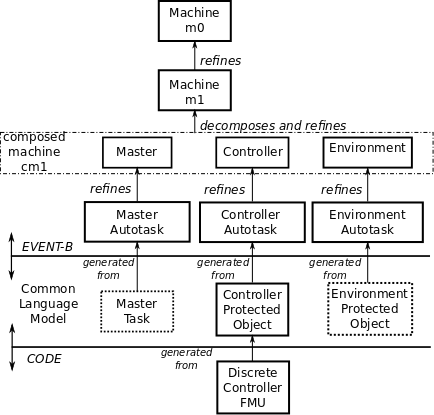
\includegraphics[width=0.9\textwidth]{devel.png}
\caption{The Code Generation Process}
\label{fig:CGProcess}
\end{figure}
This shows how an abstract model may be refined, decomposed, and then refined again to the implementation-level (i.e. above the horizontal line annotated with \emph{Event-B} ). The code generation phase (below this line) is a two-step process; although only a single step is visible to the user. The first step is to translate the Event-B machine to a language-neutral model, the Common Language Model (CLM). The CLM contains all of the information necessary to implement the model, such as tasks, protected objects, variables, subroutines and program-style statements. These entities represent the `structure' of the implementation; but the program-style, statements and conditions, retain the Event-B mathematical representation of expressions and predicates. These will be translated in the second phase. It is during this second step, when the source code is being generated, that templates contribute to the generated code. Notice that, in the diagram, the code generator produces a protected object, in the CLM, from the FMU Controller Autotask.  This is another place where code generation for FMU-C differs from our previous work. It is also the case that no code is required from the master, or environment models; this is shown in the diagram;

\section{Templates: for Configuration and Re-use}\label{templates}
%
We have already mentioned that the ADVANCE project~\cite{advance} is providing a way to co-simulate discrete Event-B models with continuous models of the environment; using the Functional Mock-Up Interface~\cite{FMISTD}. In an extension to this work we developed a code generation approach; where discrete Event-B controller models can be translated into C code, for use in FMU simulation of discrete implementations. The FMUs can then be used for simulation and testing, with models of its continuous environment. We were able to re-use much of the generator code from the existing OpenMP generator, and just provide a new FMU-C specific generator.  

When generating code from Tasking Event-B, we found that there was a large amount of boiler-plate code, from the FMI API, that we did not want to hard-code. We thought that this provided a good opportunity to explore the use of templates in code generation. Templates provide a way to re-use this `boiler-plate' code. It is also easily customised, so this is where we can make use of it for system configuration. In the first instance we surveyed the existing technology, such as Java Emitter Templates (JET)~\cite{JET}. We found that this provided a very expressive solution, but was unnecessarily complex for our simple needs. We provide an architectural overview of out template-driven approach in the diagram of Fig.~\ref{fig:templates}.
%
\begin{figure}
\centering
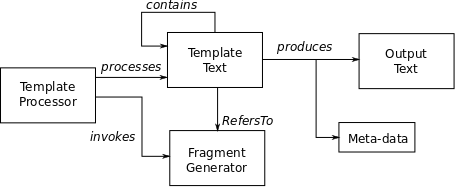
\includegraphics[width=0.8\textwidth]{templateOverview.png}
\caption{Overview of Template Use}
\label{fig:templates}
\end{figure}
%
\subsection{A Template Example}
In Fig.~\ref{fig:templates} we see the artefacts involved in template processing; namely text-based templates, code-fragment generators, text output, meta-data output and a template-processor that does the work. The templates may contain plain-text (which is copied verbatim to the target during processing) and tags. The tags may refer to other templates, or code-fragment generators. The code-fragment generators are hard-coded generators that relate to certain aspects of the final output; for instance, a fragment generator inserts the variable initialisations as specified in a template. We can see an example of this in~\ref{fig:templateExample}. 
%
\begin{figure}
\begin{center}
\begin{minipage}{0.8\textwidth}
//\#\# $<$addToHeader$>$\\
fmiStatus fmiInitializeSlave(fmiComponent c,\\
\hspace*{0.2cm}fmiReal relativeTolerance, fmiReal tStart,\\
\hspace*{0.2cm}fmiBoolean stopTimeDefined, fmiReal tStop)\{\\
\hspace*{0.4cm}fmi\_Component* mc = c;\\
\hspace*{0.4cm}//\#\# $<$initialisationsList$>$\\
\hspace*{0.4cm}//\#\# $<$stateMachineProgramCounterIni$>$\\
\hspace*{0.4cm}return fmiOK;\\
\}
\end{minipage}
\end{center}
\caption{An Example Template}
\label{fig:templateExample}
\end{figure}
%
%
The template shows part of an implementation of the FMI API's \emph{fmiInitializeSlave} function; the code in the template is common to all of the FMUs that we will generate for a particular target configuration. The tags accommodate variability between models; e.g. FMUs keep track of state-variables, which may be different for each model. These state-variables correspond exactly to the variables of the system that have been modelled in Event-B. In the function shown, the first parameter is the \emph{fmiComponent}, the `instance' of the FMU that is to be initialised. The other parameters relate to the simulation life-cycle.  

As part of the code generation approach we generate an intermediate model, the Common Language Model (CLM) which is independent of the target implementation language. The fragment-generator can use the CLM, in the translation to the C source code.  In the template, we a place-holder (which we call a \emph{tag}), where we want the variable initialisation to occur. The tags in our example begin with the character string, //\#\#.  This string is customizable, since we have provided an extension point, using the Eclipse extension mechanism, for platform developers to define which characters to use as tags.  The string we chose allows the tag to be treated as a comment; so, that the remainder of the code can be syntax checked if required. This line is continued with $<$\emph{identifier}$>$ where an \emph{identifier} is supplied. A tag is usually (but not always) an insertion point; its \emph{identifier} can relate to another template (to be expanded in-line); or the name of a fragment-generator. The fragment-generator is a Java class that can be used to generate code; or meta-data that is stored for later use, in the code generation process  (see Fig.~\ref{fig:templates}). In the example we have three tags. We will show how the template processor uses the \emph{intialisationList} tag, as a code injection point to add variable initialisations, in subsection~\ref{injection}. The first tag \emph{addToHeader} identifies a generator that creates meta-data, which are used at a later stage, for generation of a header file. The last tag is not used in our example, since we have no state-machine diagrams in the model. But, if we did have state-machines in the FMU, we would generate code to implement its initial state, in this location.
%
\subsection{Template Tags and Generators}
It is possible to categorize the users of Rodin into several types of users. One such type are the `ordinary' modellers, using Event-B in smaller organisations. But for large scale use, one may have meta-modellers (to develop product lines for instance), and another level of user may instantiate models (of the product line). There may also be platform developers, that provide platform tools for use by meta-modellers, modellers and product-line implementers. The extension points that we provide allows the platform developer to provide template utilities for the other users. The first extension point \\ \emph{org.eventb.codegen.templates.tag} has been provided to allow them to specify the \emph{tagCommentCharacters}. The second, \emph{org.eventb.codegen.templates.generator} has been provided to allow them to add new \emph{tag identifiers}, and \emph{GeneratorClass}es that implement \emph{IGenerator}. The \emph{IGenerator} interface defines a single \emph{generate} method which takes an instance of \emph{IGeneratorData} as a parameter. The \emph{IGeneratorData}  is a container for  a \emph{List} of objects, used by the \emph{generate} method, when generating the code fragment. The template-processor stores the link between \emph{tag identifier} and \emph{GeneratorClass} in a \emph{GeneratorMap} (repository). By adding a new \emph{tag identifier} and providing a new generator implementation, a Rodin-user working at the implementation-level, has this new feature available for insertion into the template, to produce some specific output. 

An overview of the  templates and generators used in the FMI translation, can be seen in Fig.~\ref{fig:templateStructure} (much of the detail is omitted for brevity). The \emph{root} template is \emph{fmuTemplate.c}, from this we can navigate to all of the other templates, and generators. The root template generates variable declarations and the subroutines, and expands the main boilerplate functions in \emph{fmuOthers.c}. The \emph{fmuInstantiate} and \emph{fmuInitialise} templates generate the corresponding FMI API function implementations. From the diagram we can see that these rely on generators to do some of the translation.
%
\begin{figure}
\centering
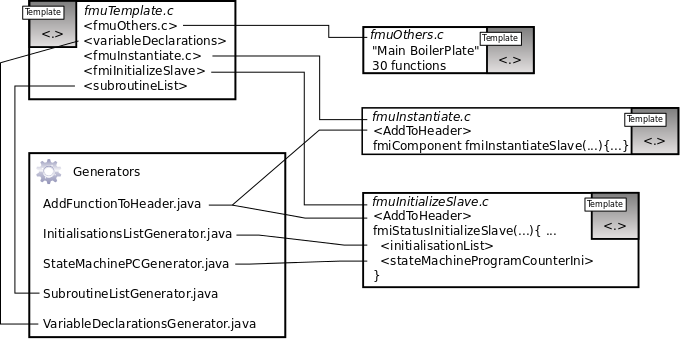
\includegraphics[width=0.9\textwidth]{templateStructure.png}
\caption{The Templates and Generators in the FMI Code Generator}
\label{fig:templateStructure}
\end{figure}
%
\subsection{Code Injection} \label{injection}
We now return to our explanation of how the \emph{initialisationList} is processed, and refer back to the example shown in Fig.~\ref{fig:templateExample}. The template-processor scans each line, and copies the output; or inserts new text, or meta-data as required, until we reach the line with the \emph{initialisationList}. The template-processor finds the \emph{initialisationList} in the \emph{GeneratorMap}. It is linked to the \emph{InitialisationListGenerator} class, by the map. The class's \emph{generate} method is invoked, to begin the process of text insertion. A fragment of the \emph{InitialisationListGenerator} class can be seen in Fig.~\ref{fig:genCode}. The class defines variables that are used to hold the data retrieved from the \emph{IGeneratorData} object;  \emph{prot} and \emph{tm} are objects that are required to process the initialisations. In this case, the declarations are retrieved from the (CLM's) \emph{Protected} object, see Fig.~\ref{fig:CGProcess}, and translated in turn.   
%
%
\begin{figure}
\centering
\begin{minipage}{0.85\textwidth}
\textbf{public class} InitialisationsListGenerator \textbf{implements} IGenerator \{\\
\hspace*{0.2cm}\textbf{public} List$<$String$>$ generate(IGeneratorData data)\{\\
\hspace*{0.4cm}List$<$String$>$ outCode = \textbf{new} ArrayList$<$String$>$();\\
\hspace*{0.4cm}Protected prot = null;\\
\hspace*{0.4cm}IL1TranslationManager tm = null;\\
\hspace*{0.4cm}\emph{//(1) Un-pack the GeneratorData}\\
\hspace*{0.4cm}List$<$Object$>$ dataList = data.getDataList();\\
\hspace*{0.4cm}\textbf{for} (Object obj : dataList) \{\\
\hspace*{0.6cm}\textbf{if} (obj instanceof Protected) \{prot = (Protected) obj;	\}\\
\hspace*{0.6cm}\textbf{else if}(obj instanceof IL1TranslationManager)\{\\
\hspace*{0.8cm}tm = (IL1TranslationManager) obj;\}\}\\
\hspace*{0.2cm}\ldots\\
\hspace*{0.2cm}\emph{//(2) Get the Declarations}\\
\hspace*{0.2cm}EList$<$Declaration$>$ declList = prot.getDecls();\\
\hspace*{0.2cm}\emph{//(3) Process each Variable Declaration/Initialisation}\\
\hspace*{0.2cm}\textbf{for} (Declaration decl : declList) \{\\
\hspace*{0.4cm}\ldots\\
\hspace*{0.4cm}String initialisation = FMUTranslator.updateFieldVariableName(\ldots);\\
\hspace*{0.4cm}outCode.add(initialisation);\\
\hspace*{0.2cm}\}\\
\hspace*{0.2cm}\emph{// (4) return the new fragment}\\
\hspace*{0.2cm}\textbf{return} outCode;\}\}
\end{minipage}
\caption{An Example Fragment-Generator}
\label{fig:genCode}
\end{figure}
%
%

The main steps are highlighted using numbered comments in the code. In step 1, the data is un-packed; in step 2, the declarations are obtained from the \emph{Protected} object; in step 3, the initialisation are translated, and add to an array of initialisation statements; in step 4, the initialisations are returned to the template-processor. The code that is generated is shown in Fig.~\ref{fig:codeOut}. 
%
\begin{figure}
\centering
\begin{minipage}{0.9\textwidth}
fmiStatus fmiInitializeSlave(fmiComponent c, fmiReal relativeTolerance,\\
\hspace*{0.6cm}fmiReal tStart, fmiBoolean stopTimeDefined, fmiReal tStop) \{\\
\hspace*{0.2cm}fmi\_Component* mc = c;\\
\hspace*{0.2cm}\emph{// (1) Injected By InitialisationsListGenerator $>>>$ }\\
\hspace*{0.2cm}mc-$>$i[c\_level\_controllerImpl\_] = 100;\\
\hspace*{0.2cm}mc-$>$b[c\_pumpOnReq\_controllerImpl\_] = fmiFalse;\\
\hspace*{0.2cm}mc-$>$b[c\_pumpOnCmd\_controllerImpl\_] = fmiFalse;\\
\hspace*{0.2cm}\ldots\\
\hspace*{0.2cm}\emph{// (2) $<<<$ End of Injection}\\
\hspace*{0.2cm}\textbf{return} fmiOK;\\
\}
\end{minipage}
\caption{The fmiInitializeSlave Function with Injected Code}
\label{fig:codeOut}
\end{figure}
%
In this code we see that variable initialisations such as:

\noindent\begin{minipage}{\textwidth}
\centering
mc-$>$i[c\_level\_controllerImpl\_] = 100;
\end{minipage}
have been generated, between the comments numbered (1) and (2). The initialisation, seen here, is very specific to the FMU approach. The variable \emph{mc}, is of type FMI component, which is an instance of an FMU. Its integer variables are stored in an array \emph{i}[]. A variable \emph{c\_level\_controllerImpl} from the model, is initialised using an index into the array \emph{c\_level\_controllerImpl\_}. This is rather complex but should demonstrate the point that we can inject code of some complexity.

%
\section{Conclusions}\label{conc}
Using the approach that we have described in this paper, we are able to perform some deploy-time target configuration, tailoring the generated code to a specific target. To do this we provide an extensible mechanism, to process the templates. The template approach also has the advantage that we can re-use boiler-plate code, and do this without having to hard-code large sections of it. The template-processor that we provide iterates through the templates and copied the contents verbatim to a target file, unless a template tag is encountered. The default usage is for the tag to refer to another template, which is processed and expanded in-line. A platform developer is able to enrich the template language, by adding new template tags and associating them with custom fragment-generators. In this way complex code generation activities can be performed, to generate text output; or meta-data in other formats. The meta-data is useful for downstream code generation. This approach also provides some scope for applying configuration options. One use might be to define different scheduling algorithms, and inject the generated code. The templates could also be modified, on-the-fly, during code generation. Exploration of these ideas is left for future research. 

During preliminary investigations we considered the following template processing approaches; Acceleo~\cite{acceleo} , Xpand~\cite{xpand}, and JET~\cite{JET}. Each of the approaches are more complex than we really need. We have also found, in previous approaches, that too much reliance on external tools can lead to integration and maintenance problems. Our own code generation approach already has many dependencies on external plug-ins, we will only increase this number if absolutely necessary. It is also the case, with these template based processors, that complex code generation control structures are difficult to use; and this is why we developed the simple interface, as a priority.  For those reasons we chose to implement our own lightweight, extensible template language and code-injection mechanism. We do recognize, however, that the burden of complexity has been shifted to the \emph{IGenerator} implementers. But, we believe this should be an acceptable trade-off, when developing a product-line for instance. 
%
\bibliographystyle{plain}
\bibliography{MyBibTex}
%
%
%
\end{document}
